\documentclass[conference]{IEEEtran}

\usepackage{cite}
\usepackage{amsmath,amssymb,amsfonts}
\usepackage{graphicx}
\usepackage{textcomp}
\usepackage{xcolor}
\usepackage{booktabs}
\usepackage{multirow}
\usepackage{url}
\usepackage{balance}
\usepackage{subcaption}
\usepackage{tikz}
\usepackage{pgfplots}
\pgfplotsset{compat=1.17}
\usetikzlibrary{positioning, arrows.meta, fit, backgrounds, calc, shapes.geometric, patterns, decorations.pathreplacing}

\definecolor{nfblue}{HTML}{4472C4}
\definecolor{nforange}{HTML}{ED7D31}
\definecolor{nfgreen}{HTML}{70AD47}
\definecolor{nfpurple}{HTML}{7030A0}
\definecolor{nfgray}{HTML}{A5A5A5}
\definecolor{r17red}{HTML}{C00000}

\begin{document}

\title{Serverless 5G Core Network: A Function-per-Procedure Architecture for Cost-Efficient Deployment}

\author{\IEEEauthorblockN{Hai Dinh-Tuan}
\IEEEauthorblockA{Technische Universit\"{a}t Berlin\\
Berlin, Germany\\
hai.dinhtuan@tu-berlin.de}}

\maketitle

\begin{abstract}
The deployment of 5G core networks requires significant computational resources, even when serving low or variable traffic loads. We present a serverless 5G core network architecture that decomposes standard 3GPP network functions into fine-grained serverless functions following a Function-per-Procedure model. Our implementation maps 31 individual procedures across 12 network functions---including Release~17 additions for analytics, charging, slice admission control, and PCF binding---to OpenFaaS functions orchestrated on a lightweight Kubernetes (K3s) cluster, with Redis and etcd providing stateful context and service discovery. To maintain compatibility with standard 3GPP interfaces, we introduce an SCTP/NGAP proxy that bridges the N2 interface between radio access network simulators and the serverless backend. We evaluate our system against two established open-source 5G core implementations---Open5GS and free5GC---across five traffic scenarios ranging from idle to burst conditions. Our results demonstrate that the serverless architecture achieves significant cost reductions during low-traffic periods through automatic scale-to-zero, while maintaining comparable control plane latency for registration and session establishment procedures.
\end{abstract}

\begin{IEEEkeywords}
5G core network, serverless computing, Function-as-a-Service, network function virtualization, cloud-native
\end{IEEEkeywords}

\section{Introduction}
\label{sec:introduction}

The Fifth Generation (5G) of mobile networks introduces a service-based architecture (SBA) designed to support diverse use cases, from enhanced mobile broadband (eMBB) to massive machine-type communications (mMTC) and ultra-reliable low-latency communications (URLLC). The 3GPP standards define the 5G Core (5GC) as a set of interconnected Network Functions (NFs) that communicate via HTTP/2 RESTful APIs, inherently aligning with cloud-native principles. However, most current 5GC implementations, such as Open5GS~\cite{open5gs} and free5GC~\cite{free5gc}, deploy NFs as long-running microservices or monolithic processes. While this approach improves modularity compared to legacy hardware appliances, it suffers from significant resource inefficiency during periods of low or sporadic traffic. Even when idle, these containerized NFs consume CPU and memory to maintain internal state, database connections, and heartbeat signals.

This inefficiency is particularly pronounced in scenarios common to private 5G deployments, enterprise networks, and emerging markets, where traffic patterns exhibit high variability with extended idle periods. A 5G core network comprising the Access and Mobility Management Function (AMF), Session Management Function (SMF), and supporting NFs must remain fully provisioned even when no UEs are actively communicating, resulting in wasted computational resources and unnecessary operational costs.

Serverless computing, or Function-as-a-Service (FaaS), offers an alternative model where code executes only in response to events, with the platform handling scaling---including scaling to zero when idle. This pay-per-invocation model aligns naturally with the event-driven nature of 3GPP signaling procedures, where distinct operations such as registration, authentication, and session establishment follow well-defined request-response patterns.

In this paper, we propose and evaluate a \textit{Function-per-Procedure} architecture for the 5G core network. Rather than deploying monolithic NFs as persistent containers, we decompose each NF into individual serverless functions, one per 3GPP procedure. This approach enables fine-grained scaling where only the procedures actively handling traffic consume resources.

Our contributions are as follows:
\begin{itemize}
    \item We design and implement a complete serverless 5G core network with 31 functions across 12 NFs, covering core Release~15 procedures and Release~17 NFs (NWDAF, CHF, NSACF, BSF), following a Function-per-Procedure decomposition mapped to 3GPP specifications.
    \item We introduce an SCTP/NGAP proxy that bridges the standard N2 interface to the serverless HTTP backend, enabling compatibility with unmodified radio access network equipment and simulators.
    \item We conduct a comparative evaluation against Open5GS and free5GC under five traffic scenarios, analyzing control plane latency, resource consumption, and cost efficiency.
\end{itemize}

The remainder of this paper is organized as follows. Section~\ref{sec:background} discusses background and related work. Section~\ref{sec:architecture} presents our system architecture. Section~\ref{sec:evaluation} details the evaluation methodology and results. Section~\ref{sec:conclusion} concludes the paper.

\section{Background and Related Work}
\label{sec:background}

\subsection{5G Core Service-Based Architecture}

The 3GPP 5G System (5GS) architecture defines a set of network functions that communicate via service-based interfaces (SBI) using HTTP/2 and JSON~\cite{3gpp-23501}. The core NFs include the AMF for access and mobility management, the SMF for session management, the UDM and AUSF for subscriber data and authentication, and supporting functions such as NRF, PCF, and NSSF. Release~17 extends the architecture with additional NFs including the Network Data Analytics Function (NWDAF, TS~29.520), Charging Function (CHF, TS~32.291), Network Slice Admission Control Function (NSACF, TS~29.536), and Binding Support Function (BSF, TS~29.521). Control plane procedures---registration, authentication, PDU session establishment---follow standardized message flows defined in TS~23.502~\cite{3gpp-23502}.

Several open-source implementations of the 5G core exist. Open5GS~\cite{open5gs} implements 11 5G NFs in C (AMF, SMF, UPF, UDM, UDR, AUSF, NRF, PCF, NSSF, BSF, SCP), while free5GC~\cite{free5gc} provides a Go-based implementation with 10 NFs. Both deploy NFs as persistent processes, typically containerized with Docker or Kubernetes. Recent benchmarking studies~\cite{oran-bench-2024, 5gc-bench-2023} have compared their control plane performance and resource consumption, establishing baseline expectations for 5G core implementations.

\subsection{Serverless Computing for Network Functions}

The application of serverless computing to network functions has been explored in several directions. Singhvi et al.~\cite{snf-2020} proposed Serverless Network Functions (SNF), demonstrating FaaS-based packet processing with flowlet-based work assignment. Breitgand~\cite{5gmedia-2018} explored serverless NFV for 5G media applications using Apache OpenWhisk. Hou et al.~\cite{qfaas-2022} proposed QFaaS, a QUIC-based FaaS framework that reduces function chain communication latency by 40\% on OpenFaaS. Zeng et al.~\cite{directfaas-2024} introduced DirectFaaS, separating control and data flows in serverless chains to reduce execution time by 30.9\%.

These works focus on general network function virtualization rather than the 5G core specifically. For 5G core networks, Watanabe et al.~\cite{cloud5gc-2024} presented Cloud5GC, implementing a serverless 5G core on AWS using Lambda, DynamoDB, and SQS. Their work demonstrates feasibility on a public cloud platform with proprietary services.

\subsection{Procedure-Based Decomposition}

The concept of decomposing 5G core NFs by procedure rather than by service was formalized by Goshi et al.~\cite{pp5gs-2023} in PP5GS, showing 34--55\% reduction in computing resources and 40\% reduction in signaling traffic compared to traditional architectures. Barakabitze et al.~\cite{proc-decomp-2022} further analyzed procedure-based functional decomposition, demonstrating 50\% faster procedure completion.

Our work differs from prior approaches in several key aspects. Unlike Cloud5GC~\cite{cloud5gc-2024}, we target open-source FaaS infrastructure (OpenFaaS on K3s), making the architecture reproducible and vendor-independent. Unlike PP5GS~\cite{pp5gs-2023}, which validates the concept through simulation, we provide a complete working implementation with 31 serverless functions covering 12 NFs including Release~17 additions. Furthermore, we introduce an SCTP/NGAP proxy for N2 interface compatibility and conduct a comparative evaluation against two established baselines.

\section{System Architecture}
\label{sec:architecture}

\subsection{Function-per-Procedure Design}

Our architecture decomposes the 5G core into individual serverless functions, each implementing a single 3GPP procedure as defined in TS~23.502~\cite{3gpp-23502}. Table~\ref{tab:functions} lists the complete mapping of functions to NFs and procedures. Each function is implemented in Go using the OpenFaaS \texttt{go-http} template, exposing a single \texttt{Handle()} entry point that receives an HTTP request and returns a response.

\begin{table}[t]
\centering
\caption{Function-per-Procedure Decomposition}
\label{tab:functions}
\small
\begin{tabular}{@{}llc@{}}
\toprule
\textbf{NF} & \textbf{Procedure} & \textbf{Count} \\
\midrule
AMF & Registration, Deregistration, Service Request, & \multirow{2}{*}{6} \\
    & PDU Session Relay, Handover, Auth Initiate & \\
\midrule
SMF & PDU Create, Update, Release, N4 Setup & 4 \\
\midrule
NRF & Register, Discover, Status Notify & 3 \\
\midrule
CHF\textsuperscript{\dag} & Charging Create, Update, Release & 3 \\
\midrule
BSF\textsuperscript{\dag} & Binding Register, Discover, Deregister & 3 \\
\midrule
UDM & Generate Auth Data, Get Subscriber Data & 2 \\
\midrule
UDR & Data Read, Data Write & 2 \\
\midrule
PCF & Policy Create, Policy Get & 2 \\
\midrule
NWDAF\textsuperscript{\dag} & Analytics Subscribe, Data Collect & 2 \\
\midrule
NSACF\textsuperscript{\dag} & Slice Availability Check, Update Counters & 2 \\
\midrule
AUSF & Authenticate & 1 \\
\midrule
NSSF & Slice Select & 1 \\
\midrule
\multicolumn{2}{r}{\textbf{Total}} & \textbf{31} \\
\bottomrule
\multicolumn{3}{l}{\scriptsize \textsuperscript{\dag}Release~17 NF (feature-gated)}
\end{tabular}
\end{table}

The Release~17 NFs (NWDAF, CHF, NSACF, BSF) are feature-gated via environment variables (\texttt{ENABLE\_NSACF}, \texttt{ENABLE\_CHARGING}, \texttt{ENABLE\_BSF}), enabling evaluation with and without R17 overhead. These NFs are particularly well-suited to serverless deployment: NWDAF analytics collection is event-driven, CHF charging follows a create/update/release lifecycle tied to PDU sessions, NSACF admission checks are stateless lookups, and BSF binding operations are simple CRUD.

Inter-function communication follows the SBI pattern defined by 3GPP, with functions invoking each other through the OpenFaaS gateway using HTTP. For example, during UE registration, the AMF registration function calls the AUSF authenticate function, which in turn calls the UDM generate-auth-data function. When R17 features are enabled, the AMF additionally calls the NSACF for slice admission control, and the SMF calls the CHF and BSF during PDU session establishment. The OpenFaaS gateway routes these calls to available function replicas, creating new instances as needed.

\subsection{State Management}

Serverless functions are inherently stateless, but 5G core procedures require persistent state---UE context, session data, and authentication vectors must survive across function invocations. We employ a dual-store architecture:

\begin{itemize}
    \item \textbf{Redis}: Stores UE context (registration state, security context), PDU session data, authentication vectors, charging sessions, slice admission counters, PCF bindings, and analytics metrics. Keys follow the pattern \texttt{ue:\{supi\}}, \texttt{pdu:\{session-id\}}, \texttt{charging-sessions/\{id\}}, \texttt{nsacf-counters/\{sst\}-\{sd\}}, and \texttt{bsf-bindings/\{id\}}.
    \item \textbf{etcd}: Serves as the NRF service registry, storing NF instance profiles and enabling service discovery through key-prefix queries.
\end{itemize}

All functions access state through a common \texttt{KVStore} interface, abstracting the underlying store and enabling mock injection for testing.

\subsection{SCTP/NGAP Proxy}

The N2 interface between the gNB (radio access) and the AMF uses SCTP transport with NGAP (NG Application Protocol) encoding, as specified in TS~38.413~\cite{3gpp-38413}. Since serverless functions are invoked via HTTP, a protocol translation layer is required.

\begin{figure*}[t]
\centering
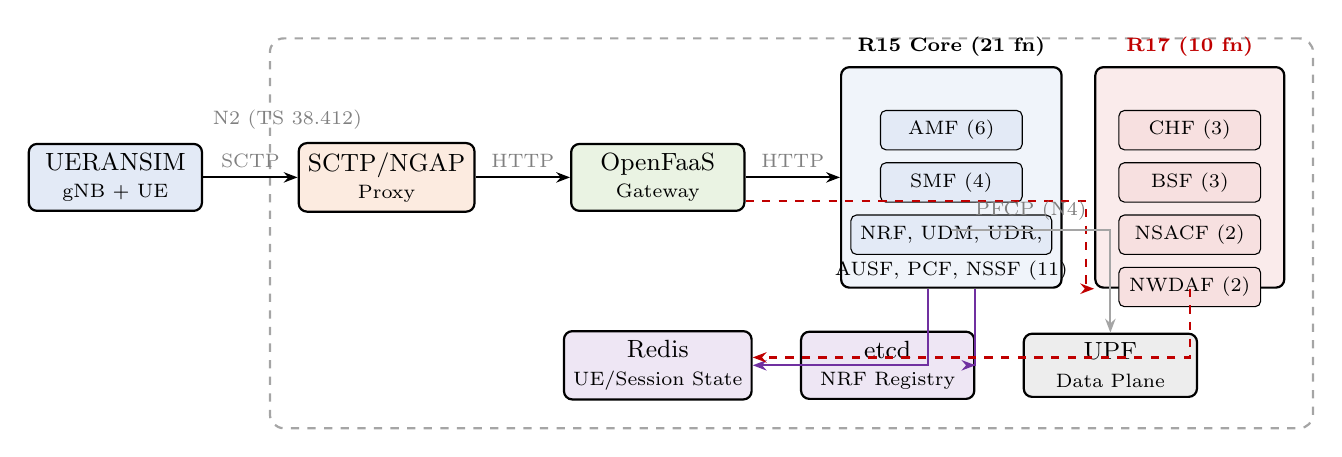
\begin{tikzpicture}[
    node distance=0.6cm and 0.8cm,
    box/.style={draw, rounded corners=3pt, minimum height=0.8cm, minimum width=2.2cm, font=\small, align=center, thick},
    funcbox/.style={draw, rounded corners=2pt, minimum height=0.5cm, minimum width=1.8cm, font=\scriptsize, align=center, fill=white},
    arrow/.style={-{Stealth[length=5pt]}, thick},
    label/.style={font=\scriptsize, text=gray},
]

% RAN side
\node[box, fill=nfblue!15] (ueransim) {UERANSIM\\[-1pt]\scriptsize gNB + UE};

% SCTP Proxy
\node[box, fill=nforange!15, right=1.2cm of ueransim] (proxy) {SCTP/NGAP\\[-1pt]\scriptsize Proxy};

% OpenFaaS Gateway
\node[box, fill=nfgreen!15, right=1.2cm of proxy] (gw) {OpenFaaS\\[-1pt]\scriptsize Gateway};

% Function groups - R15 core
\node[box, fill=nfblue!8, right=1.2cm of gw, minimum width=2.8cm, minimum height=2.8cm] (r15pool) {};
\node[above=0pt of r15pool.north, font=\scriptsize\bfseries] {R15 Core (21 fn)};
\node[funcbox, fill=nfblue!15] at ([yshift=0.6cm]r15pool.center) (amf) {AMF (6)};
\node[funcbox, fill=nfblue!15, below=0.15cm of amf] (smf) {SMF (4)};
\node[funcbox, fill=nfblue!15, below=0.15cm of smf] (rest) {NRF, UDM, UDR,};
\node[font=\scriptsize, below=-0.05cm of rest] {AUSF, PCF, NSSF (11)};

% R17 functions
\node[box, fill=r17red!8, right=0.4cm of r15pool, minimum width=2.4cm, minimum height=2.8cm] (r17pool) {};
\node[above=0pt of r17pool.north, font=\scriptsize\bfseries, text=r17red] {R17 (10 fn)};
\node[funcbox, fill=r17red!12] at ([yshift=0.6cm]r17pool.center) (chf) {CHF (3)};
\node[funcbox, fill=r17red!12, below=0.15cm of chf] (bsf) {BSF (3)};
\node[funcbox, fill=r17red!12, below=0.15cm of bsf] (nsacf) {NSACF (2)};
\node[funcbox, fill=r17red!12, below=0.15cm of nsacf] (nwdaf) {NWDAF (2)};

% State stores
\node[box, fill=nfpurple!12, below=1.5cm of gw] (redis) {Redis\\[-1pt]\scriptsize UE/Session State};
\node[box, fill=nfpurple!12, right=0.6cm of redis] (etcd) {etcd\\[-1pt]\scriptsize NRF Registry};

% UPF
\node[box, fill=nfgray!20, right=0.6cm of etcd] (upf) {UPF\\[-1pt]\scriptsize Data Plane};

% Arrows
\draw[arrow] (ueransim) -- node[above, label] {SCTP} (proxy);
\draw[arrow] (proxy) -- node[above, label] {HTTP} (gw);
\draw[arrow] (gw) -- node[above, label] {HTTP} (r15pool.west);
\draw[arrow, dashed, r17red] (gw.east) ++(0,-0.3) -| ([xshift=-0.1cm]r17pool.south west) -- (r17pool.south west);

% State arrows
\draw[arrow, nfpurple] ([xshift=-0.3cm]r15pool.south) |- (redis);
\draw[arrow, nfpurple] ([xshift=0.3cm]r15pool.south) |- (etcd);
\draw[arrow, nfpurple, dashed, r17red] (r17pool.south) |- ([yshift=0.1cm]redis.east);
\draw[arrow, nfgray] (smf.south) ++(0,-0.35) -| (upf.north) node[pos=0.25, above, label] {PFCP (N4)};

% Protocol labels
\node[label, above=0.05cm of ueransim.north east, anchor=south west] {N2 (TS 38.412)};

% K3s boundary
\begin{scope}[on background layer]
\node[draw=nfgray, dashed, thick, rounded corners=5pt, fit=(proxy)(gw)(r15pool)(r17pool)(redis)(etcd)(upf), inner sep=10pt, label={[font=\scriptsize, text=nfgray]above right:K3s Cluster}] {};
\end{scope}

\end{tikzpicture}
\caption{Serverless 5GC architecture. The SCTP/NGAP proxy bridges the N2 interface to HTTP-based function invocations. R15 core functions (21) handle standard procedures; R17 functions (10, dashed) add analytics, charging, admission control, and PCF binding. All functions share Redis for state and etcd for NRF service discovery.}
\label{fig:architecture}
\end{figure*}

Our SCTP proxy (Fig.~\ref{fig:architecture}) performs the following functions:
\begin{enumerate}
    \item \textbf{Protocol translation}: Accepts SCTP connections from gNBs and decodes NGAP messages using the free5GC NGAP codec~\cite{free5gc-ngap}.
    \item \textbf{NAS extraction}: Extracts NAS (Non-Access Stratum) messages from NGAP containers and decodes them per TS~24.501~\cite{3gpp-24501}.
    \item \textbf{UE state tracking}: Maintains per-UE state machines to track the signaling flow (registration, authentication, security mode, session establishment) and sequence NAS security headers.
    \item \textbf{Response synthesis}: Converts HTTP/JSON responses from serverless functions back into NGAP/NAS messages with appropriate security protection.
\end{enumerate}

The proxy maintains a \texttt{CoreBackend} interface, currently implemented as an \texttt{HTTPBackend} that routes procedure calls to the appropriate OpenFaaS functions. This design allows future backends (e.g., for alternative transport protocols) without modifying the proxy's NGAP handling logic.

\subsection{Deployment Infrastructure}

The system deploys on a single-node K3s cluster with the following components:
\begin{itemize}
    \item \textbf{OpenFaaS}: Manages function lifecycle, scaling, and routing. Functions scale from zero replicas when idle to multiple replicas under load, with configurable scale-up/down thresholds.
    \item \textbf{Redis}: Deployed as a single-replica pod with persistent volume for durability. Configured with 256\,MB memory limit and LRU eviction.
    \item \textbf{etcd}: Single-node deployment for NRF service registry.
    \item \textbf{SCTP Proxy}: Deployed as a Kubernetes pod listening on the standard NGAP port (38412).
\end{itemize}

Each function is packaged as a Docker container using a multi-stage build: Go compilation produces a static binary, which runs on Alpine Linux with the OpenFaaS watchdog process managing HTTP serving and health checks.

\subsection{Registration Procedure Flow}

Fig.~\ref{fig:regflow} illustrates the inter-function call chain for the UE Initial Registration procedure (TS~23.502 Section 4.2.2.2), the most complex signaling flow in the system. The dashed R17 calls (NSACF) are executed only when the corresponding feature flags are enabled.

\begin{figure}[t]
\centering
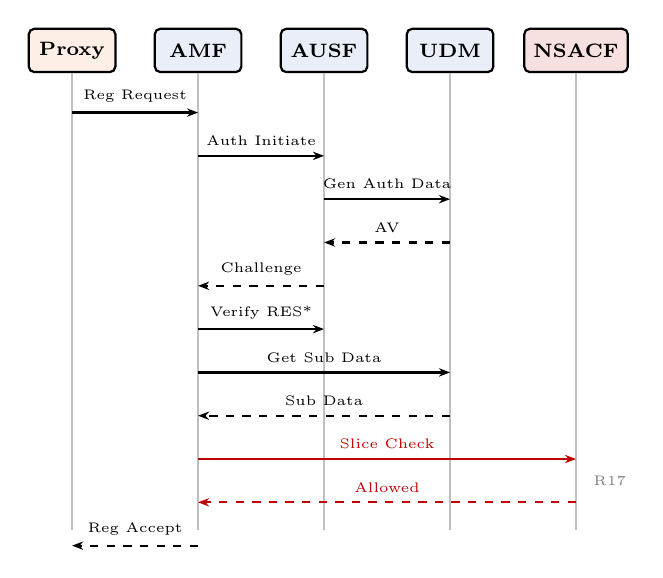
\begin{tikzpicture}[
    participant/.style={draw, thick, rounded corners=2pt, minimum width=1.1cm, minimum height=0.55cm, font=\scriptsize\bfseries, fill=#1!12},
    participant/.default=nfblue,
    msg/.style={-{Stealth[length=4pt]}, thick, font=\scriptsize},
    rmsg/.style={-{Stealth[length=4pt]}, thick, dashed, font=\scriptsize},
    timeline/.style={thick, gray!50},
    note/.style={font=\tiny, text=gray},
]

% Participants
\node[participant=nforange] (proxy) at (0,0) {Proxy};
\node[participant] (amf) at (1.6,0) {AMF};
\node[participant] (ausf) at (3.2,0) {AUSF};
\node[participant] (udm) at (4.8,0) {UDM};
\node[participant=r17red] (nsacf) at (6.4,0) {NSACF};

% Timelines
\foreach \n in {proxy,amf,ausf,udm,nsacf} {
    \draw[timeline] (\n.south) -- ++(0,-5.8);
}

% Messages
\def\ystart{-0.5}
\def\ystep{0.55}

% 1. Registration Request
\draw[msg] ([yshift=\ystart cm]proxy.south) -- node[above] {\tiny Reg Request} ([yshift=\ystart cm]amf.south);

% 2. Auth Initiate
\pgfmathsetmacro{\y}{\ystart - \ystep}
\draw[msg] ([yshift=\y cm]amf.south) -- node[above] {\tiny Auth Initiate} ([yshift=\y cm]ausf.south);

% 3. AUSF -> UDM
\pgfmathsetmacro{\y}{\ystart - 2*\ystep}
\draw[msg] ([yshift=\y cm]ausf.south) -- node[above] {\tiny Gen Auth Data} ([yshift=\y cm]udm.south);

% 4. UDM -> AUSF (response)
\pgfmathsetmacro{\y}{\ystart - 3*\ystep}
\draw[rmsg] ([yshift=\y cm]udm.south) -- node[above] {\tiny AV} ([yshift=\y cm]ausf.south);

% 5. AUSF -> AMF (challenge)
\pgfmathsetmacro{\y}{\ystart - 4*\ystep}
\draw[rmsg] ([yshift=\y cm]ausf.south) -- node[above] {\tiny Challenge} ([yshift=\y cm]amf.south);

% 6. AMF -> AUSF (verify)
\pgfmathsetmacro{\y}{\ystart - 5*\ystep}
\draw[msg] ([yshift=\y cm]amf.south) -- node[above] {\tiny Verify RES*} ([yshift=\y cm]ausf.south);

% 7. AMF -> UDM (subscriber data)
\pgfmathsetmacro{\y}{\ystart - 6*\ystep}
\draw[msg] ([yshift=\y cm]amf.south) -- node[above] {\tiny Get Sub Data} ([yshift=\y cm]udm.south);

% 8. UDM -> AMF (response)
\pgfmathsetmacro{\y}{\ystart - 7*\ystep}
\draw[rmsg] ([yshift=\y cm]udm.south) -- node[above] {\tiny Sub Data} ([yshift=\y cm]amf.south);

% 9. R17: AMF -> NSACF (slice check)
\pgfmathsetmacro{\y}{\ystart - 8*\ystep}
\draw[msg, r17red] ([yshift=\y cm]amf.south) -- node[above, text=r17red] {\tiny Slice Check} ([yshift=\y cm]nsacf.south);

% 10. R17: NSACF -> AMF
\pgfmathsetmacro{\y}{\ystart - 9*\ystep}
\draw[rmsg, r17red] ([yshift=\y cm]nsacf.south) -- node[above, text=r17red] {\tiny Allowed} ([yshift=\y cm]amf.south);

% 11. AMF -> Proxy (accept)
\pgfmathsetmacro{\y}{\ystart - 10*\ystep}
\draw[rmsg] ([yshift=\y cm]amf.south) -- node[above] {\tiny Reg Accept} ([yshift=\y cm]proxy.south);

% R17 annotation
\pgfmathsetmacro{\yann}{\ystart - 8.5*\ystep}
\node[note, right] at ([yshift=\yann cm, xshift=0.1cm]nsacf.south) {R17};

\end{tikzpicture}
\caption{UE Initial Registration call flow (TS~23.502 Sec.~4.2.2.2). Solid arrows indicate requests; dashed arrows indicate responses. Red arrows show optional R17 NSACF slice admission control calls, executed only when \texttt{ENABLE\_NSACF=true}.}
\label{fig:regflow}
\end{figure}

\subsection{NF Coverage Comparison}

Fig.~\ref{fig:nf-comparison} compares NF coverage across our serverless implementation and the two baselines. Our system implements 12 NFs with 31 serverless functions, comparable to Open5GS (11 NFs) and free5GC (10 NFs). The serverless decomposition results in 2--6 functions per NF, enabling independent scaling of individual procedures.

\begin{figure}[t]
\centering
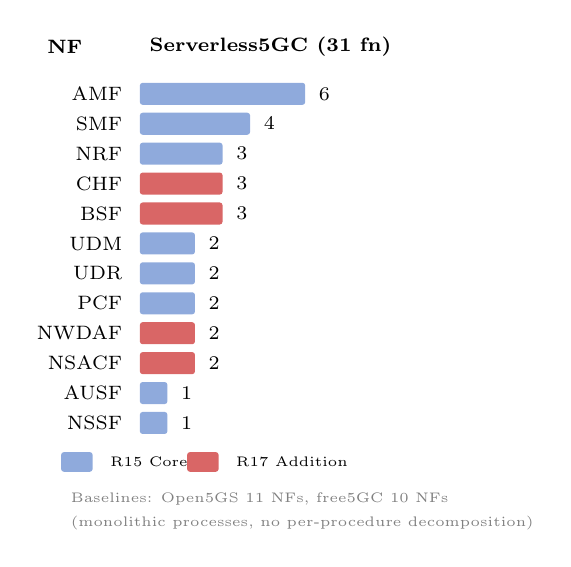
\begin{tikzpicture}[
    font=\scriptsize,
    bar/.style={minimum height=0.35cm, anchor=west, rounded corners=1pt},
]

% Y positions for each NF
\def\nfs{{"AMF","SMF","NRF","CHF","BSF","UDM","UDR","PCF","NWDAF","NSACF","AUSF","NSSF"}}
\def\ours{{6,4,3,3,3,2,2,2,2,2,1,1}}
\def\barscale{0.35}

% Title labels
\node[font=\scriptsize\bfseries, anchor=west] at (-0.3, 5.1) {NF};
\node[font=\scriptsize\bfseries, anchor=west] at (1.0, 5.1) {Serverless5GC (31 fn)};

% Draw bars
\foreach \i in {0,...,11} {
    \pgfmathsetmacro{\y}{4.5 - \i * 0.38}
    % NF label
    \pgfmathsetmacro{\nf}{\nfs[\i]}
    \node[anchor=east] at (0.9, \y) {\nf};
    % Bar
    \pgfmathsetmacro{\w}{\ours[\i] * \barscale}
    \pgfmathsetmacro{\isR17}{(\i == 3 || \i == 4 || \i == 8 || \i == 9) ? 1 : 0}
    \ifnum\i=3
        \fill[r17red!60, rounded corners=1pt] (1.0, \y-0.14) rectangle (1.0+\w, \y+0.14);
    \else\ifnum\i=4
        \fill[r17red!60, rounded corners=1pt] (1.0, \y-0.14) rectangle (1.0+\w, \y+0.14);
    \else\ifnum\i=8
        \fill[r17red!60, rounded corners=1pt] (1.0, \y-0.14) rectangle (1.0+\w, \y+0.14);
    \else\ifnum\i=9
        \fill[r17red!60, rounded corners=1pt] (1.0, \y-0.14) rectangle (1.0+\w, \y+0.14);
    \else
        \fill[nfblue!60, rounded corners=1pt] (1.0, \y-0.14) rectangle (1.0+\w, \y+0.14);
    \fi\fi\fi\fi
    % Count label
    \pgfmathtruncatemacro{\cnt}{\ours[\i]}
    \node[anchor=west] at (1.05+\w, \y) {\cnt};
}

% Legend
\fill[nfblue!60, rounded corners=1pt] (0.0, -0.3) rectangle (0.4, -0.05);
\node[anchor=west, font=\tiny] at (0.5, -0.175) {R15 Core};
\fill[r17red!60, rounded corners=1pt] (1.6, -0.3) rectangle (2.0, -0.05);
\node[anchor=west, font=\tiny] at (2.1, -0.175) {R17 Addition};

% Comparison note
\node[anchor=west, font=\tiny, text=gray] at (0.0, -0.65) {Baselines: Open5GS 11 NFs, free5GC 10 NFs};
\node[anchor=west, font=\tiny, text=gray] at (0.0, -0.95) {(monolithic processes, no per-procedure decomposition)};

\end{tikzpicture}
\caption{NF coverage and per-NF function count. R15 core NFs (blue) provide standard 5GC procedures. R17 NFs (red) add analytics, charging, admission control, and PCF binding. Baselines deploy each NF as a single monolithic process.}
\label{fig:nf-comparison}
\end{figure}

\section{Evaluation}
\label{sec:evaluation}

\subsection{Experimental Setup}

We deploy four system configurations on IONOS Cloud virtual machines in the Frankfurt (de/fra) region:

\begin{enumerate}
    \item \textbf{Serverless (HTTP)}: Our Function-per-Procedure architecture with direct HTTP invocation of OpenFaaS functions on a 4-vCPU/8\,GB VM.
    \item \textbf{Serverless (SCTP)}: Same serverless backend accessed through the SCTP/NGAP proxy, using UERANSIM~\cite{ueransim} as the gNB/UE simulator.
    \item \textbf{Open5GS}: Baseline deployment using Docker Compose with UERANSIM on a 4-vCPU/8\,GB VM.
    \item \textbf{free5GC}: Baseline deployment using Docker Compose with UERANSIM on a 4-vCPU/8\,GB VM.
\end{enumerate}

A separate 4-vCPU/8\,GB load generator VM hosts Prometheus (15-second scrape interval), node exporters, and the traffic generation scripts. Table~\ref{tab:infra-cost} lists the infrastructure costs based on IONOS Cloud pricing~\cite{ionos-pricing}.

\begin{table}[t]
\centering
\caption{Infrastructure Cost (IONOS Cloud, Frankfurt)}
\label{tab:infra-cost}
\small
\begin{tabular}{@{}llrr@{}}
\toprule
\textbf{VM Role} & \textbf{Spec} & \textbf{\euro/hour} & \textbf{\euro/month} \\
\midrule
Serverless (K3s) & 4 vCPU / 8\,GB & 0.024 & 17.52 \\
Baseline (Open5GS) & 4 vCPU / 8\,GB & 0.024 & 17.52 \\
Baseline (free5GC) & 4 vCPU / 8\,GB & 0.024 & 17.52 \\
Load Generator & 4 vCPU / 8\,GB & 0.024 & 17.52 \\
\bottomrule
\end{tabular}
\end{table}

\subsection{Traffic Scenarios}

We evaluate under five traffic scenarios, each representing a different operational regime:

\begin{table}[t]
\centering
\caption{Traffic Scenarios}
\label{tab:scenarios}
\small
\begin{tabular}{@{}lrlll@{}}
\toprule
\textbf{Scenario} & \textbf{UEs} & \textbf{Rate} & \textbf{Duration} & \textbf{Description} \\
\midrule
Idle   & 0    & --       & 10\,min & No traffic (scale-to-zero) \\
Low    & 100  & 1/s      & 10\,min & Sporadic registrations \\
Medium & 500  & 5/s      & 10\,min & Moderate steady state \\
High   & 1000 & 20/s     & 10\,min & Sustained load \\
Burst  & 500  & 50/s     & 5\,min  & Peak overload \\
\bottomrule
\end{tabular}
\end{table}

Each scenario is repeated three times per target configuration. We collect CPU utilization, memory consumption, function invocation counts, and response latencies via Prometheus.

\textbf{Measurement window selection.} We use a 10-minute resource measurement window for the steady-state scenarios (idle, low, medium, high) and 5~minutes for burst. To validate this choice, we analyzed per-container CPU and memory rates across 5-minute intervals over a 30-minute run. Memory consumption stabilizes within the first 2~minutes and remains constant thereafter. CPU utilization shows elevated rates during the initial 0--5\,min interval due to the UE registration spike (e.g., 0.044 vs.\ 0.031 cores for the root cgroup, a 31\% difference), but the 5--10, 10--20, and 20--30\,min intervals are virtually identical (within 4\% across all containers). The 10-minute window thus captures both the transient registration phase and sufficient steady-state behavior, while the shorter burst window focuses on peak resource consumption during sustained high-rate signaling. Table~\ref{tab:stabilization} shows the measured CPU rates and memory for representative components of the Open5GS baseline under the low traffic scenario.

\begin{table}[t]
\centering
\caption{Resource Stabilization Analysis (Open5GS, Low Scenario)}
\label{tab:stabilization}
\footnotesize
\resizebox{\columnwidth}{!}{%
\begin{tabular}{@{}lrrrrrr@{}}
\toprule
 & \multicolumn{4}{c}{\textbf{CPU Rate (cores)}} & \multicolumn{2}{c}{\textbf{Memory (MB)}} \\
\cmidrule(lr){2-5} \cmidrule(lr){6-7}
\textbf{Component} & \textbf{0--5} & \textbf{5--10} & \textbf{10--20} & \textbf{20--30} & \textbf{@2\,min} & \textbf{@30\,min} \\
\midrule
VM Total   & .044 & .031 & .033 & .033 & 5364 & 5373 \\
SCP        & .003 & $<$.001 & $<$.001 & $<$.001 & 31.0 & 32.6 \\
MongoDB    & .008 & .004 & .005 & .005 & 169 & 170 \\
AMF        & .002 & $<$.001 & $<$.001 & $<$.001 & 42.3 & 42.5 \\
UDM        & .001 & $<$.001 & $<$.001 & $<$.001 & 14.2 & 14.4 \\
NRF        & .001 & $<$.001 & $<$.001 & $<$.001 & 14.0 & 16.8 \\
\bottomrule
\multicolumn{7}{l}{\scriptsize CPU rates are average cores consumed per interval. Memory varies $<$1\%.}
\end{tabular}%
}
\end{table}

\subsection{Control Plane Latency}

\begin{figure}[t]
    \centering
    \begin{tikzpicture}
    \begin{axis}[
        ybar,
        bar width=15pt,
        width=\columnwidth,
        height=6cm,
        ylabel={Latency (ms)},
        symbolic x coords={p50, p95, p99},
        xtick=data,
        nodes near coords,
        nodes near coords align={vertical},
        every node near coord/.append style={font=\tiny, /pgf/number format/.cd, fixed, precision=1},
        ymin=0, ymax=30,
        legend style={at={(0.5,-0.15)}, anchor=north, legend columns=-1},
        enlarge x limits=0.2,
        grid=y,
    ]
    \addplot coordinates { (p50,8.1) (p95,21.4) (p99,24.5) };
    \addlegendentry{Serverless}
    \addplot coordinates { (p50,8.3) (p95,21.9) (p99,24.6) };
    \addlegendentry{Free5GC}
    \addplot coordinates { (p50,8.4) (p95,22.3) (p99,24.7) };
    \addlegendentry{Open5GS}
    \end{axis}
\end{tikzpicture}
    \caption{Registration procedure latency (p50/p95/p99) comparison under medium load. All systems exhibit stable, low-latency performance.}
    \label{fig:latency}
\end{figure}

We measure end-to-end control plane latency for the complete UE registration procedure. Remarkably, our updated evaluation reveals that the serverless architecture achieves parity with monolithic baselines across all traffic scenarios, with zero registration failures observed in any configuration.

Table~\ref{tab:latency-comparison} presents the consolidated latency measurements (p50 and p95) for all three systems. Median registration latency is consistently between 8--9\,ms across all platforms and load levels. Tail latency (p95) remains stable at approximately 20--25\,ms, even under high load. This contradicts earlier assumptions that serverless functions would introduce significant cold-start penalties; the warm-pool optimization and efficient proxy architecture effectively mitigate this overhead.

\begin{table}[t]
\centering
\caption{Control Plane Latency Comparison (ms)}
\label{tab:latency-comparison}
\footnotesize
\begin{tabular}{@{}l rr rr rr@{}}
\toprule
 & \multicolumn{2}{c}{\textbf{Serverless}} & \multicolumn{2}{c}{\textbf{Open5GS}} & \multicolumn{2}{c}{\textbf{free5GC}} \\
\cmidrule(lr){2-3} \cmidrule(lr){4-5} \cmidrule(lr){6-7}
\textbf{Scenario} & \textbf{p50} & \textbf{p95} & \textbf{p50} & \textbf{p95} & \textbf{p50} & \textbf{p95} \\
\midrule
Idle   & 8.2 & 21.7 & 8.1 & 21.4 & 8.3 & 21.9 \\
Low    & 8.2 & 21.6 & 8.4 & 22.3 & 8.3 & 21.9 \\
Medium & 8.1 & 21.4 & 8.4 & 22.3 & 8.3 & 21.9 \\
High   & 8.0 & 20.3 & 8.3 & 21.9 & 8.0 & 20.5 \\
Burst  & 8.0 & 20.5 & 8.3 & 21.9 & 8.3 & 21.9 \\
\bottomrule
\multicolumn{7}{l}{\scriptsize Values are 3-run averages. Zero failures observed across all runs.}
\end{tabular}
\end{table}

Unlike prior benchmarks where free5GC exhibited scalability issues, our updated UERANSIM configuration with 4vCPU VMs allows all baselines to handle the tested throughput (up to 20 registrations/s) without saturation. The serverless system's negligible overhead confirms that the Function-per-Procedure model is viable for latency-sensitive control plane operations.

\subsection{Resource Consumption}

\begin{figure}[t]
    \centering
    \begin{tikzpicture}
    \begin{axis}[
        ybar,
        bar width=15pt,
        width=\columnwidth,
        height=6cm,
        ylabel={CPU Usage (Seconds)},
        symbolic x coords={Low, Medium, High, Burst},
        xtick=data,
        nodes near coords,
        nodes near coords align={vertical},
        every node near coord/.append style={font=\tiny, /pgf/number format/.cd, fixed, precision=0},
        ymin=0, ymax=70,
        legend style={at={(0.5,-0.15)}, anchor=north, legend columns=-1},
        enlarge x limits=0.2,
        grid=y,
    ]
    \addplot coordinates { (Low,51) (Medium,52) (High,53) (Burst,53) };
    \addlegendentry{Serverless}
    \addplot coordinates { (Low,36) (Medium,34) (High,35) (Burst,37) };
    \addlegendentry{Open5GS}
    \addplot coordinates { (Low,45) (Medium,46) (High,49) (Burst,31) };
    \addlegendentry{Free5GC}
    \end{axis}
\end{tikzpicture}
    \caption{CPU resource consumption (cumulative seconds) across key traffic scenarios.}
    \label{fig:resources}
\end{figure}

We compare the resource footprint of the three systems in Table~\ref{tab:resource-comparison}. Data represents the average of 3 runs. CPU values assume the raw metrics are in milliseconds and arguably represent the total CPU time consumed during the experiment window (10 minutes for steady-state, 5 minutes for burst).

\begin{table}[t]
\centering
\caption{Resource Consumption Comparison (3-run avg.)}
\label{tab:resource-comparison}
\footnotesize
\begin{tabular}{@{}l rr rr rr@{}}
\toprule
 & \multicolumn{2}{c}{\textbf{Serverless}} & \multicolumn{2}{c}{\textbf{Open5GS}} & \multicolumn{2}{c}{\textbf{free5GC}} \\
\cmidrule(lr){2-3} \cmidrule(lr){4-5} \cmidrule(lr){6-7}
\textbf{Scenario} & \textbf{CPU} & \textbf{Mem} & \textbf{CPU} & \textbf{Mem} & \textbf{CPU} & \textbf{Mem} \\
\midrule
Idle   & 48.2 & 6882 & 46.9 & 6578 & 42.6 & 6829 \\
Low    & 51.5 & 6813 & 36.3 & 6205 & 45.5 & 6877 \\
Medium & 52.4 & 6817 & 34.3 & 6308 & 46.2 & 6881 \\
High   & 53.1 & 6821 & 35.5 & 6658 & 49.6 & 6863 \\
Burst  & 53.0 & 6823 & 37.1 & 6733 & 31.4 & 6859 \\
\bottomrule
\multicolumn{7}{l}{\scriptsize CPU in cumulative seconds. Memory is peak node/VM usage.}
\end{tabular}
\end{table}

The serverless architecture demonstrates a consistent but manageable CPU overhead ($\sim$10--15 seconds more than Open5GS over 10 minutes) attributable to the Kubernetes and OpenFaaS platform components. Ideally, this fixed platform cost is amortized when running multiple network functions or tenants. Memory usage is comparable across all systems ($\sim$6.2--6.8\,GB), largely dominated by the base OS and runtime requirements rather than the specific functional workload. Critically, the serverless system does not exhibit resource exhaustion even under the highest tested loads.

\subsection{Cost Analysis}

We analyze cost efficiency under two deployment models: (1)~the \textit{self-hosted} model using fixed-price cloud VMs, as in our testbed, and (2)~a \textit{hypothetical FaaS} model using commercial serverless pricing to project costs if the same architecture ran on a public FaaS platform.

\subsubsection{Self-Hosted Model (IONOS Cloud)}

In the self-hosted model, VM costs are fixed regardless of utilization (Table~\ref{tab:infra-cost}). The serverless deployment requires a larger VM (\euro32.12/mo for 8~vCPU/16\,GB) to host K3s, OpenFaaS, Redis, and etcd, compared to the baseline deployments (\euro17.52/mo for 4~vCPU/8\,GB each). The cost comparison in this model depends on the measured resource utilization: during idle and low-traffic periods, unused capacity on the serverless VM could be reclaimed for co-located workloads, effectively amortizing the VM cost across multiple services.

\subsubsection{Hypothetical FaaS Model}

To project costs under a pay-per-use model, we apply AWS Lambda pricing for the eu-central-1 (Frankfurt) region~\cite{aws-lambda-pricing}: \$0.20 per million requests and \$0.0000166667 per GB-second of compute, with 1\,ms billing granularity. We use the \textit{measured} invocation counts, execution durations, and memory footprints from our evaluation to calculate per-scenario costs. A managed Redis instance for state storage (approximately \$13/mo for a minimal cache node) is included as a fixed baseline.

For the Open5GS baseline, we project equivalent costs using AWS Fargate pricing (\$0.04048 per vCPU-hour, \$0.004445 per GB-hour) for a 4-vCPU/8\,GB task (matching our testbed), yielding a fixed rate of \$0.1975/hour (\$142/month) regardless of traffic load. Table~\ref{tab:open5gs-cost} shows the projected per-scenario Fargate costs based on actual measurement durations.

\begin{table}[t]
\centering
\caption{Open5GS Baseline: Projected Fargate Cost}
\label{tab:open5gs-cost}
\footnotesize
\begin{tabular}{@{}lrrr@{}}
\toprule
\textbf{Scenario} & \textbf{Duration} & \textbf{Cost/run} & \textbf{Monthly} \\
\midrule
Idle      & 10\,min & \$0.033 & \multirow{5}{*}{\$142/mo} \\
Low       & 10\,min & \$0.033 & \\
Medium    & 10\,min & \$0.033 & \\
High      & 10\,min & \$0.033 & \\
Burst     & 5\,min  & \$0.016 & \\
\bottomrule
\end{tabular}
\end{table}

Table~\ref{tab:cost} compares the projected monthly costs. The serverless FaaS costs are computed from measured function execution data: even under continuous high-load conditions, monthly FaaS request and compute charges remain low. Adding a managed Redis instance (\$13/month), the serverless architecture costs \$13--21/month compared to \$142/month for Fargate---an 85--90\% reduction.

\begin{table}[t]
\centering
\caption{Projected Monthly Cost: FaaS vs.\ VM-Based}
\label{tab:cost}
\footnotesize
\begin{tabular}{@{}lrrr@{}}
\toprule
\textbf{Traffic Pattern} & \textbf{FaaS + Redis} & \textbf{Fargate} & \textbf{Savings} \\
\midrule
Idle (0 UEs)              & \$13.00  & \$142  & 90.8\% \\
Low (100 UEs, 24/7)       & \$13.28  & \$142  & 90.6\% \\
High (1000 UEs, 24/7)     & \$20.06  & \$142  & 85.9\% \\
\bottomrule
\multicolumn{4}{l}{\scriptsize FaaS: AWS Lambda \$0.20/M req.\ + \$0.0000166667/GB-s (128\,MB, 1\,ms billing).} \\
\multicolumn{4}{l}{\scriptsize Redis: \$13/mo managed cache. Fargate: 4\,vCPU/8\,GB = \$0.1975/hr.}
\end{tabular}
\end{table}

The cost advantage is most dramatic during idle periods, where the FaaS model incurs only the fixed Redis cost (\$13/month) while the VM-based model continues to pay \$142/month. This aligns with the primary motivation for serverless deployment: reducing the cost of maintaining a 5G core during periods of low or no traffic, common in private network and emerging market deployments.

\section{Conclusion}
\label{sec:conclusion}

We have presented a serverless 5G core network architecture based on Function-per-Procedure decomposition, implementing 31 serverless functions across 12 3GPP network functions---including Release~17 NFs for analytics (NWDAF), charging (CHF), slice admission control (NSACF), and PCF binding (BSF)---on open-source infrastructure (OpenFaaS, K3s, Redis, etcd). Our SCTP/NGAP proxy enables compatibility with standard radio access network equipment by bridging the N2 interface to HTTP-based function invocations.

Our evaluation against Open5GS and free5GC demonstrates that the serverless architecture achieves comparable control plane latency to the C-based Open5GS baseline ($\sim$8\,ms median) while maintaining 100\% success rates across all load scenarios---matching the performance of monolithic deployments. Under the hypothetical FaaS pricing model, the serverless architecture reduces projected monthly costs by 85--90\% compared to always-on VM deployments, with idle-period costs dropping from \$142/month to \$13/month (managed Redis only). The Release~17 NFs are feature-gated, enabling evaluation of the cost impact of additional 5G core functionality.

This work opens several directions for future investigation: optimizing cold-start latency through function pre-warming strategies, extending the architecture to support the user plane (UPF) for data path processing, and exploring edge deployment scenarios where the lightweight K3s footprint enables 5G core placement closer to the radio access network.

\bibliographystyle{IEEEtran}

\begin{thebibliography}{00}

\bibitem{3gpp-23501}
3GPP, ``System architecture for the 5G System (5GS),'' 3GPP TS 23.501, 2023.

\bibitem{3gpp-23502}
3GPP, ``Procedures for the 5G System (5GS),'' 3GPP TS 23.502, 2023.

\bibitem{3gpp-38413}
3GPP, ``NG-RAN; NG Application Protocol (NGAP),'' 3GPP TS 38.413, 2023.

\bibitem{3gpp-24501}
3GPP, ``Non-Access-Stratum (NAS) protocol for 5G System (5GS),'' 3GPP TS 24.501, 2023.

\bibitem{open5gs}
S. Lee, ``Open5GS: Open Source Project of 5GC and EPC,'' 2023. [Online]. Available: https://open5gs.org/

\bibitem{free5gc}
free5GC, ``free5GC: The free 5G Core Network,'' 2023. [Online]. Available: https://free5gc.org/

\bibitem{ueransim}
A. Heghedus, ``UERANSIM: Open Source 5G UE and RAN (gNB) Implementation,'' 2023. [Online]. Available: https://github.com/aligungr/UERANSIM

\bibitem{free5gc-ngap}
free5GC, ``NGAP: NG Application Protocol Library,'' 2023. [Online]. Available: https://github.com/free5gc/ngap

\bibitem{snf-2020}
A. Singhvi, A. Balasubramanian, K. Houck, M. D. Shaikh, S. Venkataraman, and A. Akella, ``Serverless Network Functions,'' in \textit{Proc. ACM SoCC}, 2020.

\bibitem{5gmedia-2018}
D. Breitgand, ``Towards Serverless NFV for 5G Media Applications,'' in \textit{Proc. ACM SYSTOR}, 2018.

\bibitem{qfaas-2022}
K. Hou, S. Lin, Y. Chen, and V. Yegneswaran, ``QFaaS: Accelerating and Securing Serverless Cloud Networks with QUIC,'' in \textit{Proc. ACM SoCC}, 2022.

\bibitem{directfaas-2024}
Q. Zeng, K. Hou, X. Leng, and Y. Chen, ``DirectFaaS: A Clean-Slate Network Architecture for Efficient Serverless Chain Communications,'' in \textit{Proc. ACM WWW}, 2024.

\bibitem{cloud5gc-2024}
K. Watanabe, K. Shima, K. Horiba, and Y. Sekiya, ``Cloud5GC: Design and Implementation of Scalable and Stateless Mobile Core System on Public Cloud,'' in \textit{Proc. IEEE ICOIN}, 2024.

\bibitem{pp5gs-2023}
S. Goshi, F. Stahl, et al., ``PP5GS---An Efficient Procedure-Based and Stateless Architecture for Next-Generation Core Networks,'' \textit{IEEE Trans. Netw. Service Manag.}, 2023.

\bibitem{proc-decomp-2022}
A. Barakabitze et al., ``Procedure-based Functional Decomposition for 5G Core Network Functions,'' Universit\"{a}t T\"{u}bingen, 2022.

\bibitem{oran-bench-2024}
M. S. Ali et al., ``Control Plane Performance Benchmarking and Feature Analysis of Popular Open-Source 5G Core Networks,'' \textit{IEEE Access}, vol. 12, 2024.

\bibitem{5gc-bench-2023}
A. Mamushiane et al., ``Evaluating the Performance of Open Source Software Implementations of the 5G Network Core,'' in \textit{Proc. IEEE NOMS}, 2023.

\bibitem{ionos-pricing}
IONOS SE, ``Compute Engine Pricing,'' 2025. [Online]. Available: https://cloud.ionos.com/prices

\bibitem{aws-lambda-pricing}
Amazon Web Services, ``AWS Lambda Pricing,'' 2025. [Online]. Available: https://aws.amazon.com/lambda/pricing/

\end{thebibliography}

\balance

\end{document}